\documentclass[10pt]{beamer}

\setbeamercovered{dynamic} %para que salgan suaves los items ya pasados o por pasar
\usetheme{bars}
\usecolortheme{crane}
%I would like serif fonts for the body, but not the outline. cant figure out how to do that right now though.
\usefonttheme[onlymath]{serif}
%\setbeamerfont{sidebar}{family=\sffamily}
%\setbeamerfont{infolines}{family=\sffamily}

\usepackage{beamerthemesplit}

\title{\textbf{Superconductivity and Electron Tunneling}}
\author{Thomas McColgan y Miguel Garc\'ia Echevarr\'ia}
\institute{\emph{Laboratorio de Bajas Temperaturas \\
		Dpto. de F\'isica de la Materia Condensada} \\
		Universidad Aut\'onoma de Madrid\\
		\vspace{0.3cm}
		
\includegraphics[height=1cm]{logo}
		}
\date{Madrid, 26 de Mayo de 2008}

\begin{document}

\frame{\titlepage}

\section{Introducci\'on}
\frame{\tableofcontents}

%---------------------------------------------------------------------------
\begin{frame}
\frametitle{Un poco de historia...}

\begin{columns}
\begin{column}{0.5\textwidth}
	\begin{itemize}
		\item{Teor\'ia BCS $\longrightarrow$ Existe un gap de energ\'ia}
		\item{Medidas indirectas}
		\item{Giaever lo consigue medir directamente}
		\item{Premio Nobel en 1973}
	\end{itemize}
\end{column}
\begin{column}{0.5\textwidth}
	\begin{figure}[!h] \label{giaever60}
	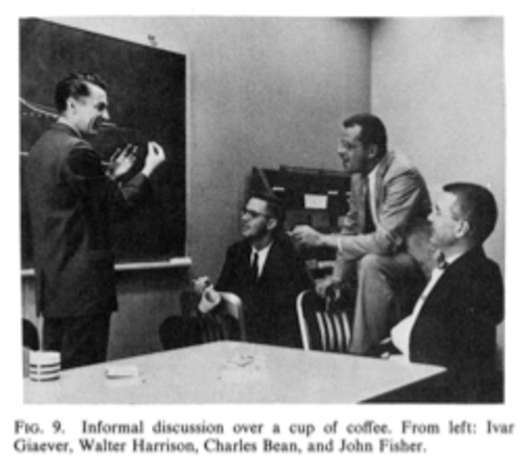
\includegraphics[width=0.6\textwidth]{giaever60}
	\end{figure}
	\begin{figure}[!h] \label{giaever99}
	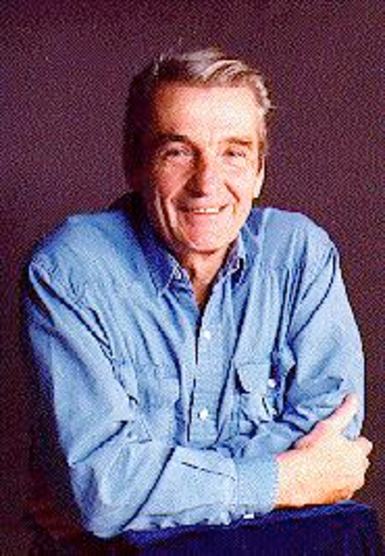
\includegraphics[width=0.4\textwidth]{giaever99}
	\end{figure}
\end{column}
\end{columns}

\end{frame}
 %---------------------------------------------------------------------------  
%---------------------------------------------------------------------------
\begin{frame}
\frametitle{Objetivos}

\begin{itemize}
	\item{Produce Samples}
	\item{Measure Current}
	\item{Calculate Gap}
\end{itemize}

\end{frame}
%---------------------------------------------------------------------------

\section{Teor\'ia}
%---------------------------------------------------------------------------------------
\begin{frame}
\frametitle{Efecto t�nel cu�ntico}
Explicar simplemente el efecto t�nel cu�ntico... 

F�rmula, quiz� s�lo la dependencia de la anchura y del potencial...

\end{frame}
%---------------------------------------------------------------------------------------
%---------------------------------------------------------------------------------------
\begin{frame}
\frametitle{}

\end{frame}
%---------------------------------------------------------------------------------------
%---------------------------------------------------------------------------------------
\begin{frame}
\frametitle{}

\end{frame}
%---------------------------------------------------------------------------------------
%---------------------------------------------------------------------------------------
\begin{frame}
\frametitle{Densidad de estados para los 3 tipos de uniones}

\begin{figure}[h!]
\centering
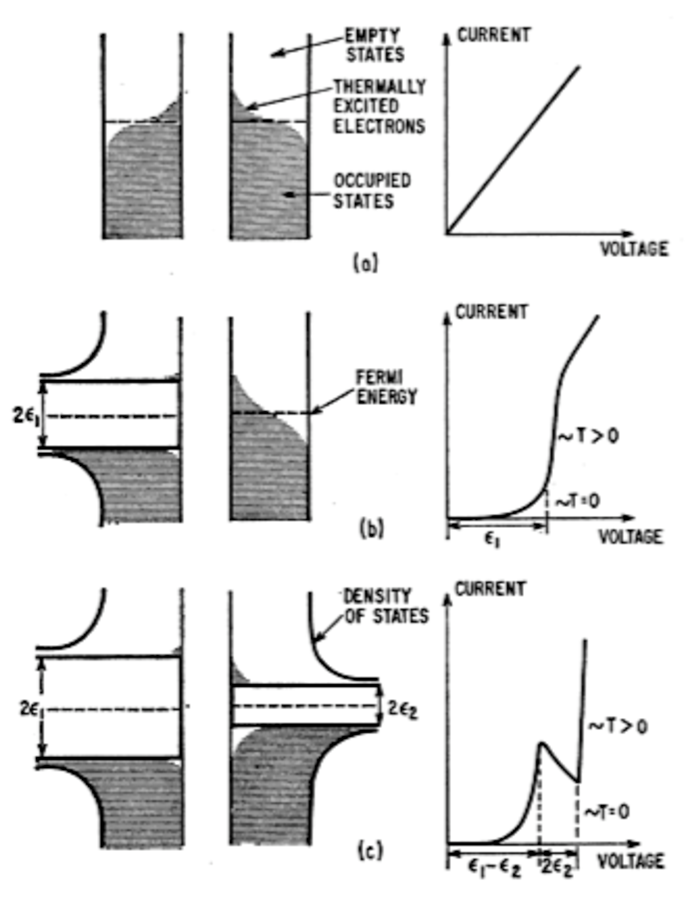
\includegraphics[width=0.6\textwidth]{fermi_levels}
%\caption{\small Densidad de estados para los 3 casos
%\label{fermi_levels}}
\end{figure}

\end{frame}
%---------------------------------------------------------------------------------------
%---------------------------------------------------------------------------------------
\begin{frame}
\frametitle{}

\end{frame}
%---------------------------------------------------------------------------------------
%---------------------------------------------------------------------------------------
\begin{frame}
\frametitle{}

\end{frame}
%---------------------------------------------------------------------------------------
%---------------------------------------------------------------------------------------
\begin{frame}
\frametitle{}

\end{frame}
%---------------------------------------------------------------------------------------
%---------------------------------------------------------------------------------------
\begin{frame}
\frametitle{}

\end{frame}
%---------------------------------------------------------------------------------------
%---------------------------------------------------------------------------------------
\begin{frame}
\frametitle{}

\end{frame}
%---------------------------------------------------------------------------------------

\section{M\'etodo experimental}

%Slide Preparation

%thickness estimation

%Cryostat

%Measurement
  %4 teminales

\section{An\'alisis y Resultados}
%----------------------------------------------------------------------------
%----------------------------------------------------------------------------
\frame
{
  \frametitle{Integraci\'on y Diferenciaci\'on Num\'ericas}
   
   \begin{itemize}
     \item<1-> Derivamos ajustando una recta a $n$ puntos consecutivos. La pendiente aproxima la derivada.
     \item<2-> Este m\'etodo tambi\'en suaviza los datos.
     \item<3-> Nunca tenemos $\frac{\Delta I}{\Delta V}=0$ porque $\Delta I>0$
     \item<4-> Tambi\'en tenemos que integrar
     \begin{equation*}\label{ins}
		I^{NS} = \frac{C^{NN}}{e} \int_{-\infty}^{\infty} dE\ \frac{|E|}{\sqrt{E^2-\Delta^2}} [f(E-eV)-f(E)]
	\end{equation*}
     \item<5-> Lo hacemos anal\'iticamente para $|E-\Delta|$ peque\~nos y numericamente para $|E-\Delta|\to\infty$
   \end{itemize}
  
}

%----------------------------------------------------------------------------
%----------------------------------------------------------------------------
\frame
{
  \frametitle{Diferencias al Modelo BCS}
  
      \begin{columns}
\begin{column}{0.6\textwidth}

  
  \begin{itemize}
  \item<1-> El modelo BCS no predice perfectamente la densidad de estados
  \item<2-> La causa puede ser que hay interaci\'on fon\'on-electr\'on adicional
  \item<3-> Giaever tambi\'en observ\'o este efecto
  \item<4-> Debido a esta diferencia no podemos ajustar los datos autom\'aticamente.
  \end{itemize}
    \end{column}
\begin{column}{0.4\textwidth}
	\begin{figure}[!h] \label{sample}
	\includegraphics<1-2>[width=\textwidth]{gv_theo_exp_7}
	\includegraphics<3->[width=\textwidth]{phonons_giaever}
	\end{figure}
\end{column}
 \end{columns} 


\uncover<5->{\textcolor{red}{\emph{Nos resignamos a hacerlo a mano\dots}}}
}

%----------------------------------------------------------------------------
%----------------------------------------------------------------------------
\frame
{
  \frametitle{Calculando Temperatura y Conductancia}
    \begin{columns}
\begin{column}{0.6\textwidth}
    \begin{itemize}
     \item<1-> Tenemos 3 par\'ametros independientes: $T$, $C_{NN}$ y $\Delta$ 
     \item<2-> Podemos hallar $T$ y $C_{NN}$ con otras medidas
     \item<3-> Calculamos $C_{NN}$ usando medidas de conductancia a $T\gg T_C$
     \item<4-> Calculamos $T$ con las medidas de presi\'on, y la curva de presi\'on de vapor del $He$.
  \end{itemize}
  
    \end{column}
    \begin{column}{0.4\textwidth}
	\begin{figure}[!h] \label{sample}
	\includegraphics<3>[width=\textwidth]{conductance2}
	\includegraphics<4>[width=\textwidth]{vap_he}
	\end{figure}
    \end{column}
    \end{columns} 

}

%----------------------------------------------------------------------------
%----------------------------------------------------------------------------
\frame
{
  \frametitle{Ajustando el Gap}
  
      \begin{itemize}
     \item<1-> Ahora podemos ajustar $\Delta$, el gap.
     \item<2->  $\Delta$ cambia poco ($0.1 meV$) en nuestro rango de temperaturas .
     \item<3-> Intentamos ajustar un valor de  $\Delta$ para todas medidas.
     \item<4-> Encontramos un valor de $\Delta = (1.4 \pm 0.1) meV$
     \end{itemize}
}


%----------------------------------------------------------------------------
%----------------------------------------------------------------------------
\frame
{
  \frametitle{Temperaturas m\'as bajas}
    \begin{columns}
\begin{column}{0.6\textwidth}
     \begin{itemize}
      \item<1-> Nuestra \'ultima medida ten\'ia $T\approx 1.2K$
      \item<2-> Hemos encontrado una curva de conductancia muy distinta
      \item<3-> Se puede explicar con la transici\'on de partes del $Al$ a superconductor
      \item<4-> No hay conductancia negativa, as\'i que no es todo superconductor.
     \end{itemize}
     
       \end{column}
\begin{column}{0.4\textwidth}
	\begin{figure}[!h] \label{sample}
	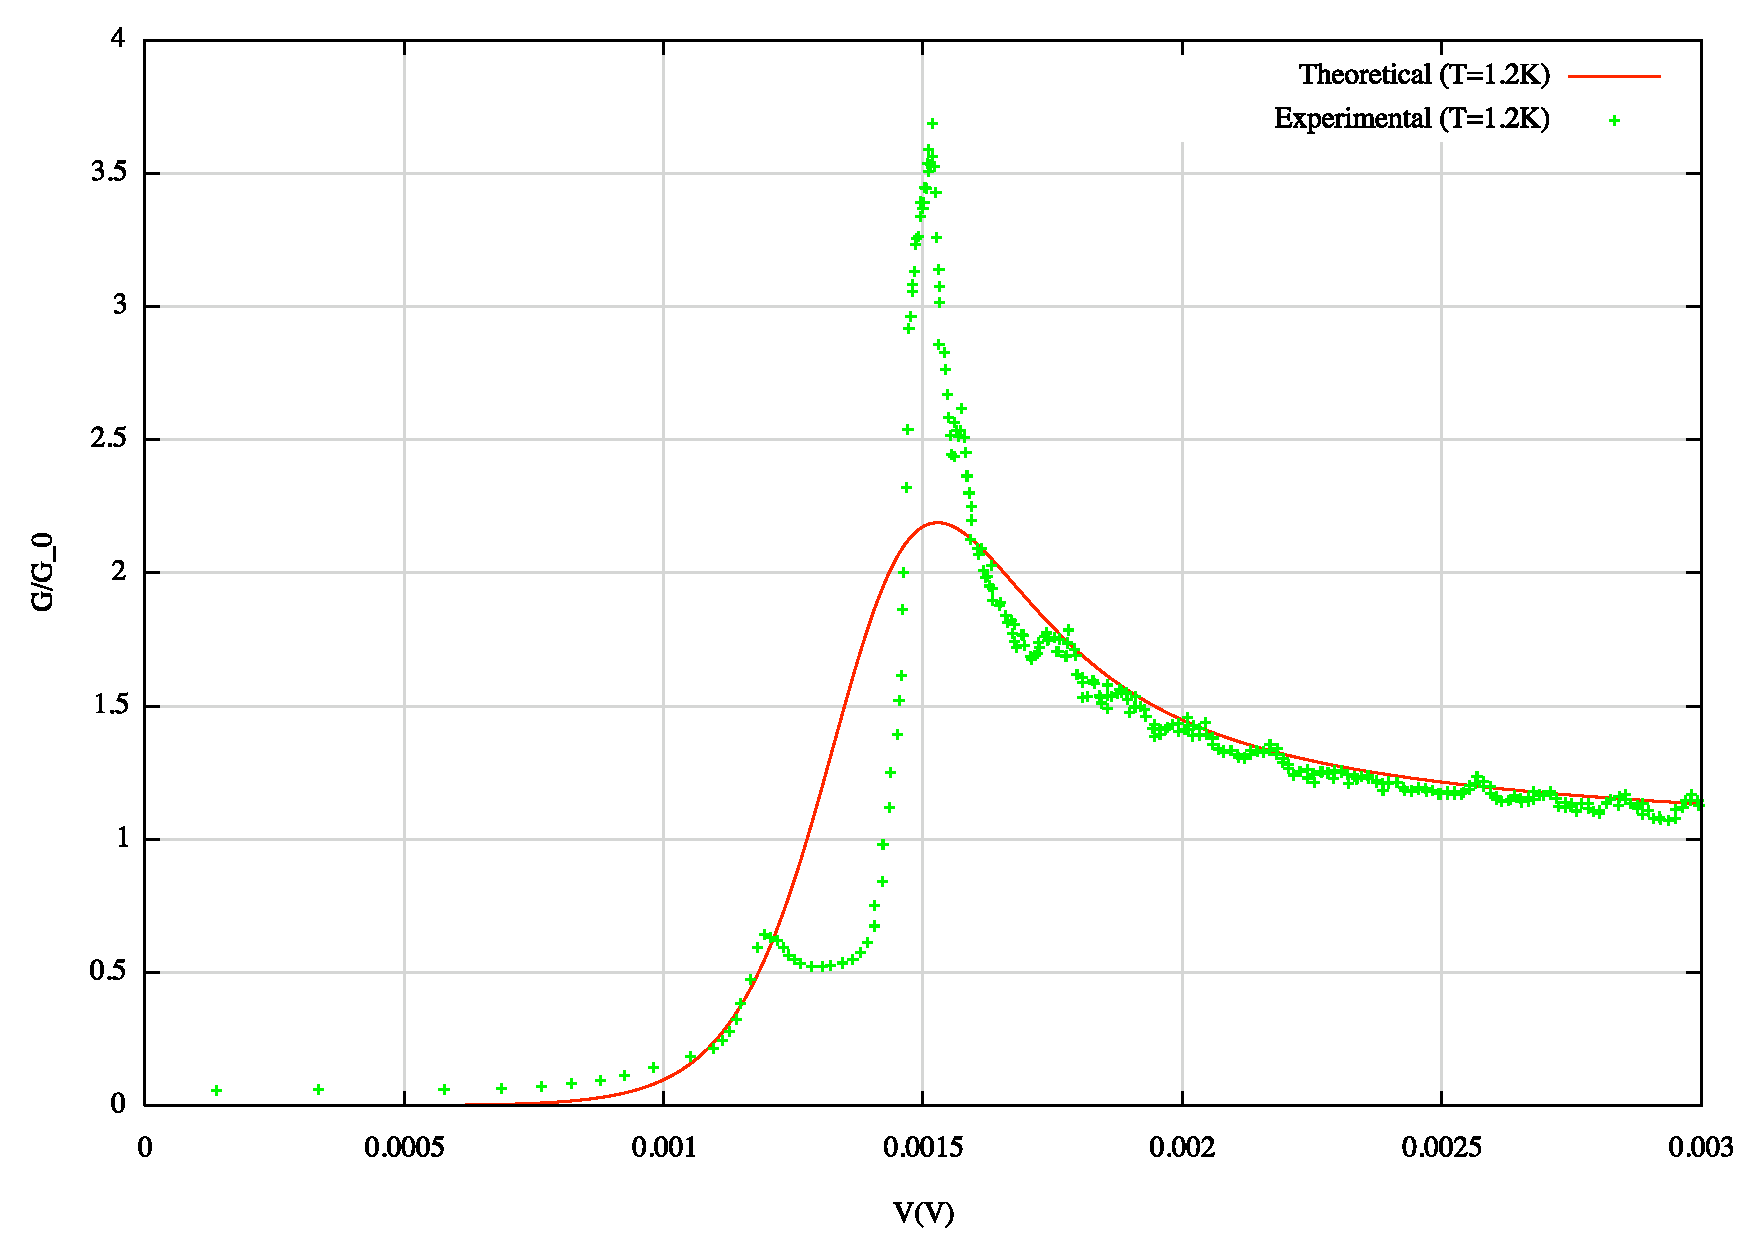
\includegraphics[width=\textwidth]{gv_theo_exp_10}
	\end{figure}
\end{column}
\end{columns} 

 }
 %----------------------------------------------------------------------------
%----------------------------------------------------------------------------



\section{Resumen y Perspectivas}
%Final Result

%Campo Magnetico

%Super-Super

%STM


\end{document}
